\documentclass[a4paper]{article}
\usepackage[a4paper,top=2cm,bottom=2cm,left=1cm,right=1cm,marginparwidth=1.75cm]{geometry}
% \usepackage[spanish]{babel}
% \selectlanguage{spanish}
% \usepackage[utf8]{inputenc}
% \usepackage[T1]{fontenc}
% \usepackage[spanish]{babel}

% \usepackage[T1]{fontenc}
\usepackage{graphicx} %Paquete para usar imagenes
\usepackage{listings}
\usepackage{xcolor}
\usepackage{tcolorbox}

\definecolor{background}{HTML}{E7EBF4}
\definecolor{bg}{HTML}{1a1b26}
\definecolor{fg}{HTML}{a9b1d6}
\definecolor{comment}{HTML}{848cb5}
\definecolor{cyan}{HTML}{82aaff}
\definecolor{orange}{HTML}{ff9e64}
\definecolor{yellow}{HTML}{e9d78e}
\definecolor{purple}{HTML}{c792ea}
\definecolor{green}{HTML}{7fdbca}
\definecolor{numbers}{HTML}{9854f1}
\definecolor{keyword}{HTML}{9854f1}

\lstset{
    showspaces=false, % Evita mostrar espacios en blanco como ␣
    showstringspaces=false,
    inputencoding=utf8,
    extendedchars=true,
    literate=%
    {á}{{\'a}}1
    {é}{{\'e}}1
    {í}{{\'i}}1
    {ó}{{\'o}}1
    {ú}{{\'u}}1
    {ñ}{{\~n}}1
}
\lstdefinestyle{mystyle}{
    language=Python,
    basicstyle=\ttfamily,
    keywordstyle=\color{keyword},
    commentstyle=\color{comment},
    numbers=none,
    numberstyle=\tiny\color{numbers},
    frame=none,
    breaklines=true,
    % showstringspaces=false
    xleftmargin=0mm,
    xrightmargin=0mm,
}

\lstset{style=mystyle}

\newtcolorbox{mycodebox}[1][]{
    arc=17pt,  % Radio de las esquinas redondeadas
    colback=background,  % Color de fondo del cuadro
    boxrule=0.5pt,  % Grosor de la línea del cuadro
    colframe=background,
    width=0.8\textwidth,   % Anchura del cuadro
    % height=5cm,            % Altura del cuadro
    % breakable,
    #1  % Otras opciones personalizadas que puedas necesitar
}


\newtcolorbox{mycodeboxl}[1][]{
    arc=7pt,  % Radio de las esquinas redondeadas
    colback=background,  % Color de fondo del cuadro
    boxrule=0.5pt,  % Grosor de la línea del cuadro
    colframe=background,
    width=0.94\textwidth,   % Anchura del cuadro
    % height=5cm,            % Altura del cuadro
    % breakable,
    #1  % Otras opciones personalizadas que puedas necesitar
}

% Documento
\begin{document}
\newgeometry{left=3cm,right=3cm,top=2cm,bottom=2cm}
\begin{titlepage}

%--------------- Nuevo comendo de linea ----------------->
\newcommand{\linea}{\rule{\linewidth}{0.7mm}} 
\center
%--------------- Universidad, facultad y carrera ----------------->
\textbf{\Large UNIVERSIDAD NACIONAL DE SAN ANTONIO ABAD DEL CUSCO}\\[0.2cm]
\textbf{\Large FACULTAD DE INGENIERÍA ELÉCTRICA, ELECTRÓNICA,INFORMÁTICA Y MECÁNICA}\\[0.2cm]
\textbf{\Large INGENIERÍA INFORMÁTICA Y DE SISTEMAS\\[0.6cm]}

%--------------- Escudos png ----------------->

\includegraphics[width=8cm]{src/escudo-unsaac.png}
\vfill

%--------------- Tema ----------------->
\linea
\\[0.3cm]
% \vfill
\textbf{\LARGE Guía de Laboratorio 6 - Reflexión}\\[0.2cm]
\linea \\
\vfill

%--------------- Integrantes ----------------->
\textit{\Large Alumno:}\\
%Integrantes del grupo
    \textbf{\large Ian Logan Will Quispe Ventura}\\
    \textit{211359}\\
    % \vfill

%--------------- Profesor y curso ----------------->
\vspace{0.3cm}
    \textit{\Large Docente:}\\
    \textbf{\large Hector Eduardo Ugarte Rojas}\\
\vspace{0.5cm}
    \textit{\Large Curso:}\\
    \textbf{\large Computación Gráfica}\\
    \vfill

\vspace{0.4cm}
    \textbf{\Large Cusco - Perú }\\
    \textbf{\large 2023 - II }\\
    \newpage
    \end{titlepage}

\restoregeometry
\newpage
% •·•·•·•·•·•••·•·•·•·•·•·•·•·•·•·•·•·•·•·•·•·•·•·•·•·•.,..,
% \section{Funcionamiento del algoritmo DDA}

\Large{\textbf{Escalado de un triángulo}}\\[-0.4cm]
\begin{center}
\begin{mycodeboxl}
\begin{lstlisting}
from OpenGL.GL import *
from OpenGL.GLUT import *
from OpenGL.GLU import *

def ptoEscaladoX(x1, x0, Sx):
    return x0 + (x1 - x0)*Sx

def ptoEscaladoY(y1, y0, Sy):
    return y0 + (y1 - y0)*Sy

def escalaTriangulo(x1, y1, x2, y2, x3, y3, Sx, Sy):
    x1e = ptoEscaladoX(x1, x3, Sx)
    y1e = ptoEscaladoY(y1, y3, Sy)
    x2e = ptoEscaladoX(x2, x3, Sx)
    y2e = ptoEscaladoY(y2, y3, Sy)

    glColor3f(0.8, 0.26, 1.0)
    glBegin(GL_LINE_LOOP)
    glVertex2f(x1, y1)
    glVertex2f(x2, y2)
    glVertex2f(x3, y3)
    glEnd()

    glColor3f (0.5 , 0.3 , 0.9)
    glBegin(GL_LINE_LOOP)
    glVertex2f(x1e, y1e)
    glVertex2f(x2e, y2e)
    glVertex2f(x3, y3)
    glEnd()
\end{lstlisting}
\end{mycodeboxl}
\end{center}
% -------------------------------------------------------------------
\newpage
\begin{center}
\begin{mycodeboxl}
\begin{lstlisting}
def display():
    x1 = 120.0
    y1 = 160.0
    x2 = 150.0
    y2 = 300.0
    x3 = 60.0
    y3 = 100.0
    Sx = 2
    Sy = 2

    glClear(GL_COLOR_BUFFER_BIT)
    escalaTriangulo(x1, y1, x2, y2, x3, y3, Sx, Sy)
    glFlush()

def myinit():
    glClearColor(1.0, 1.0, 1.0, 1.0)
    glColor3f(1.0, 0.0, 0.0)
    glPointSize(1.0)
    glMatrixMode(GL_PROJECTION)
    glLoadIdentity()
    glClearColor (0.9 ,0.92 , 0.95 , 1.0)
    gluOrtho2D(0.0, 499.0, 0.0, 499.0)

def main():
    glutInit()
    glutInitDisplayMode(GLUT_SINGLE | GLUT_RGB)
    glutInitWindowSize(500, 500)
    glutInitWindowPosition(0, 0)
    glutCreateWindow("Escalamiento")
    glutDisplayFunc(display)
    myinit()
    glutMainLoop()

if __name__ == "__main__":
    main()
\end{lstlisting}
\end{mycodeboxl}
\end{center}
\newpage
% -------------------------------------------------------------------
Gráfico generado 
\begin{center}
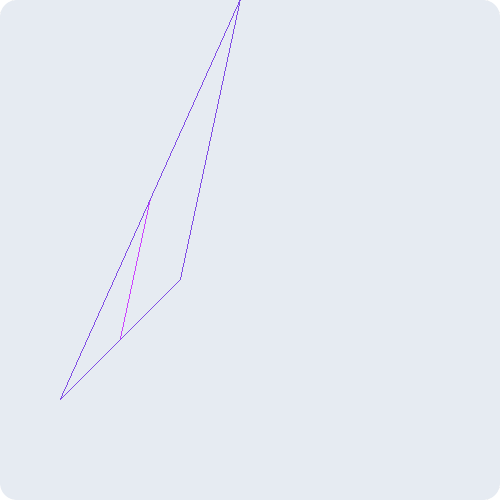
\includegraphics[width=11cm]{src/1.png}
\end{center}
\newpage
\Large{\textbf{Reflexión en el eje X}}\\[-0.4cm]
\begin{center}
\begin{mycodeboxl}
\begin{lstlisting}
from OpenGL.GL import *
from OpenGL.GLUT import *
from OpenGL.GLU import *
import sys

def reflejaTrianguloX(x1, y1, x2, y2, x3, y3):
    x1r, y1r, x2r, y2r, x3r, y3r = 0, 0, 0, 0, 0, 0
    # Dibujar ejes x e y 
    glColor3f (0.5 , 0.3 , 0.9)
    glBegin(GL_LINES)
    glVertex2f(0, 250)
    glVertex2f(500, 250)
    glVertex2f(50, 0)
    glVertex2f(50, 500)
    glEnd()
    # Puntos a nueva escala 
    x1, y1 = x1 + 50, y1 + 250
    x2, y2 = x2 + 50, y2 + 250
    x3, y3 = x3 + 50, y3 + 250
    # Dibujar triangulo original
    glColor3f(0.8, 0.26, 1.0)
    glBegin(GL_LINE_LOOP)
    glVertex2f(x1, y1)
    glVertex2f(x2, y2)
    glVertex2f(x3, y3)
    glEnd()
    # Reflejar el triangulo 
    x1r, y1r = x1, -y1 + 500
    x2r, y2r = x2, -y2 + 500
    x3r, y3r = x3, -y3 + 500
    # Dibujar el triangulo reflejado 
    glBegin(GL_LINE_LOOP)
    glVertex2f(x1r, y1r)
    glVertex2f(x2r, y2r)
    glVertex2f(x3r, y3r)
    glEnd()
\end{lstlisting}
\end{mycodeboxl}
\end{center}
% -------------------------------------------------------------------

\begin{center}
\begin{mycodebox}
\begin{lstlisting}
def display():
    x1, y1, x2, y2, x3, y3 = 120.0, 160.0, 100.0, 200.0, 10.0, 100.0
    glClear(GL_COLOR_BUFFER_BIT)

    reflejaTrianguloX(x1, y1, x2, y2, x3, y3)
    glFlush()

def myinit():
    glClearColor(1.0, 1.0, 1.0, 1.0)
    glColor3f(1.0, 0.0, 0.0)
    glPointSize(1.0)
    glMatrixMode(GL_PROJECTION)
    glLoadIdentity()
    glClearColor (0.9 ,0.92 , 0.95 , 1.0)
    gluOrtho2D(0.0, 499.0, 0.0, 499.0)

def main():
    glutInit(sys.argv)
    glutInitDisplayMode(GLUT_SINGLE | GLUT_RGB)
    glutInitWindowSize(500, 500)
    glutInitWindowPosition(0, 0)
    glutCreateWindow("Reflection")
    glutDisplayFunc(display)
    myinit()
    glutMainLoop()

if __name__ == "__main__":
    main()
\end{lstlisting}
\end{mycodebox}
\end{center}
% -------------------------------------------------------------------
\newpage
Gráfico generado\\
\begin{center}
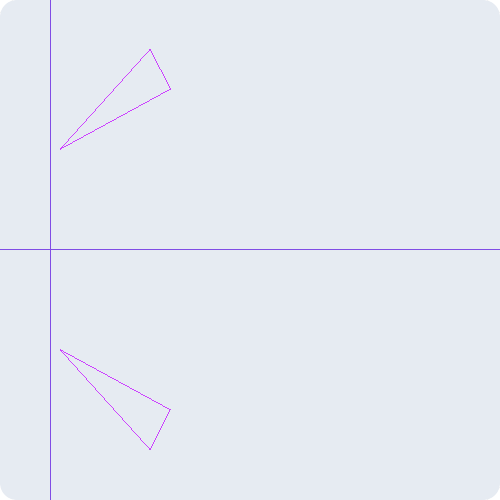
\includegraphics[width=16cm]{src/2.png}
\end{center}
\newpage


\Large{\textbf{Reflexión en el eje Y}}\\[-0.4cm]
\begin{center}
\begin{mycodeboxl}
\begin{lstlisting}
from OpenGL.GL import *
from OpenGL.GLUT import *
from OpenGL.GLU import *
import sys

def reflejaTrianguloY(x1, y1, x2, y2, x3, y3):
    x1r, y1r, x2r, y2r, x3r, y3r = 0, 0, 0, 0, 0, 0
    # Draw X and Y axes
    glColor3f (0.5 , 0.3 , 0.9)
    glBegin(GL_LINES)
    glVertex2f(250, 0)
    glVertex2f(250, 500)
    glVertex2f(0, 50)
    glVertex2f(500, 50)
    glEnd()
    # Convert points to a new scale
    x1, y1 = x1 + 250, y1 + 50
    x2, y2 = x2 + 250, y2 + 50
    x3, y3 = x3 + 250, y3 + 50
    glColor3f(0.8, 0.26, 1.0)
    # Draw the original triangle
    glBegin(GL_LINE_LOOP)
    glVertex2f(x1, y1)
    glVertex2f(x2, y2)
    glVertex2f(x3, y3)
    glEnd()
    # Reflect the triangle with respect to the Y axis
    x1r, y1r = -x1 + 500, y1
    x2r, y2r = -x2 + 500, y2
    x3r, y3r = -x3 + 500, y3
    # Draw the reflected triangle
    glBegin(GL_LINE_LOOP)
    glVertex2f(x1r, y1r)
    glVertex2f(x2r, y2r)
    glVertex2f(x3r, y3r)
    glEnd()
\end{lstlisting}
\end{mycodeboxl}
\end{center}
% -------------------------------------------------------------------
\newpage

\begin{center}
\begin{mycodeboxl}
\begin{lstlisting}
def display():
    x1, y1, x2, y2, x3, y3 = 120.0, 160.0, 100.0, 200.0, 10.0, 100.0
    glClear(GL_COLOR_BUFFER_BIT)

    reflejaTrianguloY(x1, y1, x2, y2, x3, y3)
    glFlush()

def myinit():
    glClearColor(1.0, 1.0, 1.0, 1.0)
    glColor3f(1.0, 0.0, 0.0)
    glPointSize(1.0)
    glMatrixMode(GL_PROJECTION)
    glLoadIdentity()
    glClearColor (0.9 ,0.92 , 0.95 , 1.0)
    gluOrtho2D(0.0, 499.0, 0.0, 499.0)

def main():
    glutInit(sys.argv)
    glutInitDisplayMode(GLUT_SINGLE | GLUT_RGB)
    glutInitWindowSize(500, 500)
    glutInitWindowPosition(0, 0)
    glutCreateWindow("Reflection")
    glutDisplayFunc(display)
    myinit()
    glutMainLoop()

if __name__ == "__main__":
    main()
 \end{lstlisting}
\end{mycodeboxl}
\end{center}
\newpage
Gráfico generado\\
\begin{center}

\includegraphics[width=13cm]{src/3.png}
\end{center}
\newpage
% -------------------------------------------------------------------
\Large{\textbf{Circulo escalado 2 veces manteniendo se eje fijo}}\\[-0.4cm]
\begin{center}
\begin{mycodeboxl}
\begin{lstlisting}
from OpenGL.GL import *
from OpenGL.GLUT import *
from OpenGL.GLU import *
import math

def puntoEscaladoX(x, centro_x, factor_escala_x):
    return centro_x + (x - centro_x) * factor_escala_x

def puntoEscaladoY(y, centro_y, factor_escala_y):
    return centro_y + (y - centro_y) * factor_escala_y

# Algoritmo de dibujo del círculo
def dibujarCirculo(centro_x, centro_y, radio):
    glBegin(GL_LINE_LOOP)
    for i in range(800):
        theta = 2.0 * math.pi * float(i) / float(800)
        x = centro_x + radio * math.cos(theta)
        y = centro_y + radio * math.sin(theta)
        glVertex2f(x, y)
    glEnd()

# Algoritmo de dibujo del círculo escalado
def escalaCirculo(centro_x, centro_y, radio, factor_escala_x, factor_escala_y):
    glBegin(GL_LINE_LOOP)
    for i in range(800):
        theta = 2.0 * math.pi * float(i) / float(800)
        x = centro_x + radio * math.cos(theta)
        y = centro_y + radio * math.sin(theta)
        x_escala = puntoEscaladoX(x, centro_x, factor_escala_x)
        y_escala = puntoEscaladoY(y, centro_y, factor_escala_y)
        glVertex2f(x_escala, y_escala)
    glEnd()
\end{lstlisting}
\end{mycodeboxl}
\end{center}
\newpage
\begin{center}
\begin{mycodebox}
\begin{lstlisting}
def display():
    glClear(GL_COLOR_BUFFER_BIT)
    
    # Dibujar círculo original en azul
    glColor3f (0.5 , 0.3 , 0.9)
    dibujarCirculo(250, 250, 70)
    
    # Dibujar círculo escalado en rojo
    glColor3f(0.8, 0.26, 1.0)
    escalaCirculo(250, 250, 70, 2, 2)
    
    glFlush()

def myinit():
    glClearColor(1.0, 1.0, 1.0, 1.0)
    glColor3f(1.0, 0.0, 0.0)
    glPointSize(1.0)
    glMatrixMode(GL_PROJECTION)
    glLoadIdentity()
    glClearColor (0.9 ,0.92 , 0.95 , 1.0)
    gluOrtho2D(0.0, 499.0, 0.0, 499.0)

def main():
    glutInit()
    glutInitDisplayMode(GLUT_SINGLE | GLUT_RGB)
    glutInitWindowSize(500, 500)
    glutInitWindowPosition(0, 0)
    glutCreateWindow("Escalamiento de Círculo")
    glutDisplayFunc(display)
    myinit()
    glutMainLoop()

if __name__ == "__main__":
    main()
  
\end{lstlisting}
\end{mycodebox}
\end{center}
\newpage
Gráfico generado\\
\begin{center}
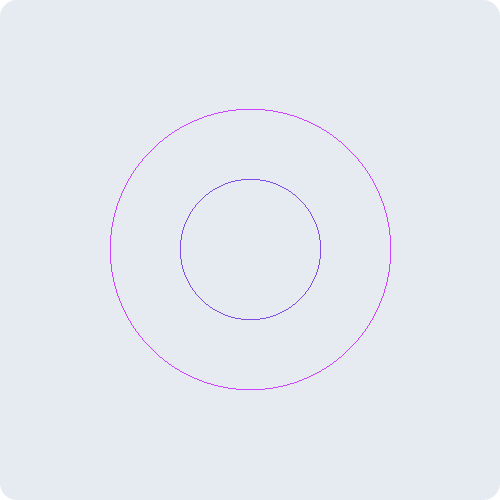
\includegraphics[width=13cm]{src/4.png}
\end{center}

\newpage
\Large{\textbf{Reflexión de un poligono de 5 lados en ek eje X}\\[-0.4cm]
\begin{center}
\begin{mycodebox}
\begin{lstlisting}
from OpenGL.GL import *
from OpenGL.GLUT import *
from OpenGL.GLU import *
import sys

# Polígono de 5 lados
def poligono(vertices):
    glBegin(GL_LINE_LOOP)
    for x, y in vertices:
        glVertex2f(x, y)
    glEnd()
def reflejoX(vertices):
    vertices_reflejados = [(x, -y + 500) for x, y in vertices]
    return vertices_reflejados
def poligono_reflejado(vertices):
    poligono(vertices)
    vertices_reflejados = reflejoX(vertices)
    poligono(vertices_reflejados)
def display():
    vertices = [(50.0, 50.0), (100.0, 150.0), (200.0, 150.0), (250.0, 50.0), (150.0, 0.0)]
    glClear(GL_COLOR_BUFFER_BIT)
    glColor3f (0.5 , 0.3 , 0.9)
    # Ejes X e Y
    glBegin(GL_LINES)
    glVertex2f(0, 250)
    glVertex2f(500, 250)
    glVertex2f(25, 0)
    glVertex2f(25, 500)
    glEnd()
    glColor3f(0.8, 0.26, 1.0)
    poligono_reflejado(vertices)
    glFlush()
\end{lstlisting}
\end{mycodebox}
\end{center}

\begin{center}
\begin{mycodebox}
\begin{lstlisting}
def myinit():
    glClearColor(1.0, 1.0, 1.0, 1.0)
    glColor3f(1.0, 0.0, 0.0)
    glPointSize(1.0)
    glMatrixMode(GL_PROJECTION)
    glLoadIdentity()
    glClearColor (0.9 ,0.92 , 0.95 , 1.0)
    gluOrtho2D(0.0, 499.0, 0.0, 499.0)

def main():
    glutInit(sys.argv)
    glutInitDisplayMode(GLUT_SINGLE | GLUT_RGB)
    glutInitWindowSize(500, 500)
    glutInitWindowPosition(0, 0)
    glutCreateWindow("Poligono de 5 lados reflejado en el eje X")
    glutDisplayFunc(display)
    myinit()
    glutMainLoop()

if __name__ == "__main__":
    main()
\end{lstlisting}
\end{mycodebox}
\end{center}
Gráfico generado\\
\begin{center}
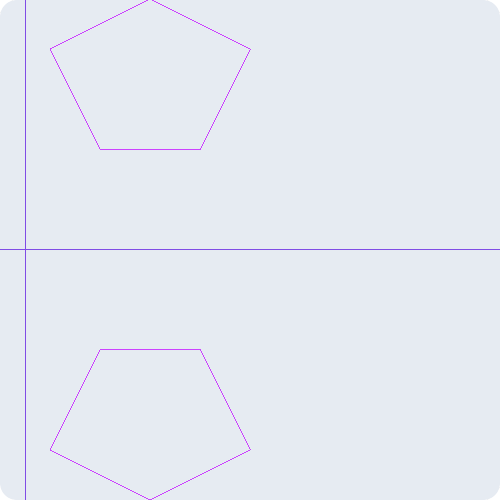
\includegraphics[width=13cm]{src/5.png}
\end{center}
\newpage
\Large{\textbf{Reflexión en los ejes X e Y}}\\[-0.4cm]
\begin{center}
\begin{mycodebox}
\begin{lstlisting}
from OpenGL.GL import *
from OpenGL.GLUT import *
from OpenGL.GLU import *
import sys

# Dibujar triangulo
def triangulo(vertices):
    glBegin(GL_LINE_LOOP)
    for x, y in vertices:
        glVertex2f(x, y)
    glEnd()

# Reflejar triangulo
def reflejar(vertices, matriz_reflexion):
    vertices_reflejados = []
    for x, y in vertices:
        x_reflejado = matriz_reflexion[0][0] * x + matriz_reflexion[0][1] * y
        y_reflejado = matriz_reflexion[1][0] * x + matriz_reflexion[1][1] * y
        vertices_reflejados.append((x_reflejado, y_reflejado))
    return vertices_reflejados

def display():
    vertices_originales = [(50.0, 50.0), (100.0, 150.0), (200.0, 150.0)]
    matrices_reflexion = [
        [[-1, 0], [0, 1]],   # Segundo cuadrante 
        [[1, 0], [0, 1]],     # Primer cuadrante 
        [[-1, 0], [0, -1]],  # Tercer cuadrante 
        [[1, 0], [0, -1]],]   # Cuarto cuadrante 
\end{lstlisting}
\end{mycodebox}
\end{center}

\begin{center}
\begin{mycodebox}
\begin{lstlisting}
    glClear(GL_COLOR_BUFFER_BIT)
    glColor3f (0.5 , 0.3 , 0.9)
    # Dibujar ejes X e Y
    glBegin(GL_LINES)
    glVertex2f(-499, 0)
    glVertex2f(499, 0)
    glVertex2f(0, -499)
    glVertex2f(0, 499)
    glEnd()
    # Dibujar el triangulo original y en los diferentes cuadrantes 
    glColor3f(0.8, 0.26, 1.0)
    for matriz in matrices_reflexion:
        vertices_reflejados = reflejar(vertices_originales, matriz)
        triangulo(vertices_reflejados)
    glFlush()
def myinit():
    glClearColor(1.0, 1.0, 1.0, 1.0)
    glColor3f(1.0, 0.0, 0.0)
    glPointSize(1.0)
    glMatrixMode(GL_PROJECTION)
    glLoadIdentity()
    glClearColor (0.9 ,0.92 , 0.95 , 1.0)
    glClearColor (0.9 ,0.92 , 0.95 , 1.0)
    # Valores negativos necesarios para los cuadrantes
    gluOrtho2D(-499.0, 499.0, -499.0, 499.0)
def main():
    glutInit(sys.argv)
    glutInitDisplayMode(GLUT_SINGLE | GLUT_RGB)
    glutInitWindowSize(500, 500)
    glutInitWindowPosition(0, 0)
    glutCreateWindow("Reflexión en ambos ejes X e Y")
    glutDisplayFunc(display)
    myinit()
    glutMainLoop()

if __name__ == "__main__":
    main()
\end{lstlisting}
\end{mycodebox}
\end{center}
Gráfico generado\\
\begin{center}
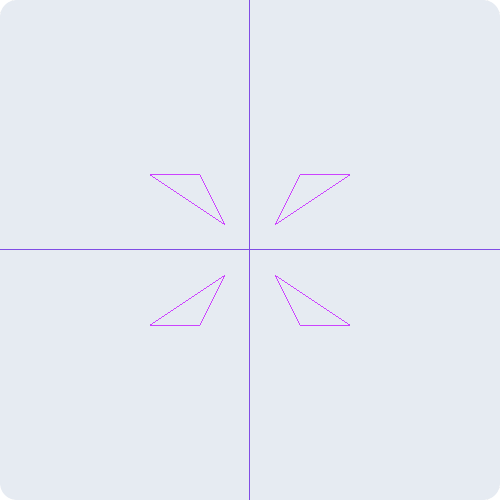
\includegraphics[width=13cm]{src/6.png}
\end{center}
\newpage
\end{document}
